\documentclass[letter,12pt,portrait]{article}

\usepackage[top=1in, bottom=1in, left=1in, right=1in]{geometry}
%\usepackage{graphicx}
\usepackage{tikz,amsmath}
\usetikzlibrary{positioning}
%\usepackage{float}
%\restylefloat{table}
\usepackage[miktex]{gnuplottex}
\usepackage{pgfplots}
\usepackage{pgfplotstable}
\pgfplotsset{compat=newest}

\begin{document}
\begin{figure}
    \centering
    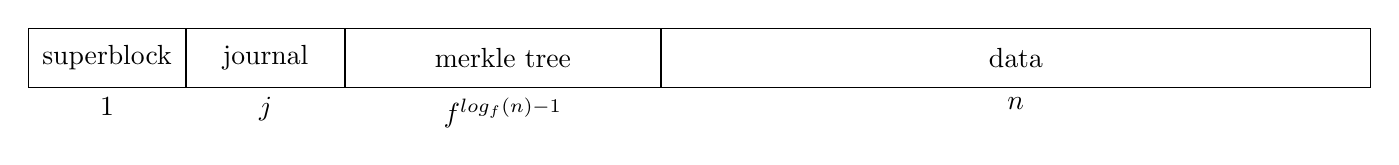
\begin{tikzpicture}
        \node(superblock)[draw,rectangle,minimum width=2cm,minimum height=0.75cm,label=below:$1$]{superblock};
        \node(journal)[right =0cm of superblock,draw,rectangle,minimum width=2cm,minimum height=0.75cm,label=below:$j$]{journal};
        \node[right =0cm of journal,draw,rectangle,minimum width=4cm,minimum height=0.75cm,label=below:$f^{log_f(n)-1}$] (metadata) (merkletree)  {merkle tree};
        \node(data) [right =0cm of merkletree,draw,rectangle,minimum width=9cm,minimum height=0.75cm,label=below:$n$] (data) {data};
    \end{tikzpicture}
    \caption{Block layout and count} \label{fig:blocks}
\end{figure}
\noindent\textbf{Variables:}
\begin{itemize}
    \item $j$ is the amount of blocks allocated for journaling
        \begin{itemize}
            \item $min(j) = \lceil\log_f(n)-1\rceil + C$
            \item $C$ is the amount of blocks for $jbd$ metadata
        \end{itemize}
    \item $f$ is the fanout of the merkle tree
        \begin{itemize}
            \item $f = \frac{block_{bits}}{hash_{bits}}$
            \item Ie, for a $4k$ block size and $sha256$, $f = \frac{4096 \cdot 8}{256} = 128$
        \end{itemize}
    \item $n$ is the amount of blocks useable by the user
\end{itemize}
\noindent\textbf{Sections:}\\
\textbf{superblock:}\\
Stores the information for the set up of a given verity instance. (Modified from original verity superblock layout)\\
%\begin{table}
\begin{tabular}{|l|l|r|}
    \hline
    \textbf{Name} & \textbf{Detail} & \textbf{Size (bytes)} \\ \hline
    signature & mint\textbackslash0\textbackslash0\textbackslash0\textbackslash0  & 8\\ \hline
    version & superblock version, 2 & 4\\ \hline
    hash\_type & 0 - Chrome OS, 1 - Normal & 4\\ \hline
    uuid & uuid of device & 16 \\ \hline
    algorithm & hash algorithm name & 32\\ \hline
    hash\_block\_size  & hash blocks in bytes & 4\\ \hline
    data\_block\_size & data blocks in bytes & 8\\ \hline
    salt\_size & salt size & 2\\ \hline
    \_pad1 & padding & 6 \\ \hline
    salt & salt & 256 \\ \hline
    %\_pad2 & padding & 168 \\ \hline
    hmac\_algorithm & hmac hash algorithm name & 32 \\ \hline
    hmac & hmac of root & 128 \\ \hline
    jbd\_block\_size & jbd blocks in bytes & 4 \\ \hline
    \_pad2 & padding & 4 \\ \hline
\end{tabular}
%\caption{Original Superblock layout}
%\end{table}
\\
\textbf{journal:}\\
Blocks allocated for $jbd$\\
\textbf{merkle tree:}\\
Merkle tree format\\
\textbf{data:}\\
Blocks allocated for user data\\

\begin{tikzpicture}
\begin{axis}[ylabel=merkle tree size (GB) , xlabel=data size (GB), title=Data size vs Merkle Tree Size,
    domain=1:4096,
    scale=2.0,
    smooth, no markers,
    enlargelimits=false,grid=major,
    ytick={0,10,20,...,60},
    xtick={0,512,1024,...,4096}
]
\addplot gnuplot {64**(log(x*262144)/log(64) - 1) / 262144}; \addlegendentry{$sha512$}
\addplot gnuplot {128**(log(x*262144)/log(128) - 1) / 262144}; \addlegendentry{$sha256$}
\addplot gnuplot {204**(log(x*262144)/log(204) - 1) / 262144}; \addlegendentry{$sha1$}
\end{axis}
\end{tikzpicture}

\begin{tikzpicture}
\begin{axis}[ylabel=merkle tree levels , xlabel=data size (GB), title=Data size vs Number of Merkle Tree Levels,
    domain=0.1:128,
    scale=2.0,
    smooth, no markers,
    enlargelimits=false,grid=major,
    ytick={0,1,2,...,6},
    xtick={0,16,32,...,128}
]
\addplot gnuplot {log(x*262144)/log(64) - 1}; \addlegendentry{$sha512$}
\addplot gnuplot {log(x*262144)/log(128) - 1}; \addlegendentry{$sha256$}
\addplot gnuplot {log(x*262144)/log(204) - 1}; \addlegendentry{$sha1$}
\end{axis}
\end{tikzpicture}

\begin{tikzpicture}
\begin{axis}[ylabel=merkle tree levels , xlabel=data size (GB), title=Data size vs Number of Merkle Tree Levels,
    domain=0.1:4096,
    scale=2.0,
    smooth, no markers,
    enlargelimits=false,grid=major,
    ytick={0,1,2,...,6},
    xtick={0,512,1024,...,4096}
]
\addplot gnuplot {log(x*262144)/log(64) - 1}; \addlegendentry{$sha512$}
\addplot gnuplot {log(x*262144)/log(128) - 1}; \addlegendentry{$sha256$}
\addplot gnuplot {log(x*262144)/log(204) - 1}; \addlegendentry{$sha1$}
\end{axis}
\end{tikzpicture}



%\begin{tikzpicture}[scale=0.1]
    %\begin{axis}[domain=0:1024]
        %\addplot gnuplot {128**(log(x)/log(128))};
    %\end{axis}
    %\tkzinit[xmax=1024,xstep=10,ymax=50, ystep=10]
    %\tkzgrid[xstep=10,ystep=10](0,0)(1024,50)
    %\draw[very thin,color=gray] (-0.1,-1.1) grid (3.9,3.9);
    %\draw[->] (-0.2,0) -- (4.2,0) node[right] {$x$};
    %\draw[->] (0,-1.2) -- (0,4.2) node[above] {$f(x)$};
    %\draw[color=red] plot[id=x] function{x} 
        %node[right] {$f(x) =x$};
    %\draw[color=blue] plot[id=sin] function{sin(x)} 
        %node[right] {$f(x) = \sin x$};
    %\draw[color=orange] plot[id=exp] function{0.05*exp(x)} 
        %node[right] {$f(x) = \frac{1}{20} \mathrm e^x$};
%\end{tikzpicture}


\end{document}
